\documentclass[10pt]{article}
\usepackage[margin=0.68in]{geometry}
\usepackage[T1]{fontenc}
\usepackage{lmodern,amsmath,graphicx,booktabs,hyperref}
\hypersetup{colorlinks=true,urlcolor=blue}
\setlength{\parindent}{0pt}\setlength{\parskip}{5pt}
\setlength{\emergencystretch}{3em}
\begin{document}
{\Large\bfseries Actual child ports and replicated packet vertices}

23 November 2026. Local only; no S3. Unsigned producer observations.
Formal PCC7df097; native PCC5429db. \texttt{[pcc:unverified]}

For one fixed coordinate, kernel and mode tuple, the actual constructor has
two different full-family identities. If the parent has $M$ edges and $V$
old vertices, with $P$ valid packets and $r$ labels, then
\[
 \sum_{g=0}^{r-1} M_g=2M,
 \qquad \sum_{g=0}^{r-1} V_g=V+rP.
\]
Parallel incidences and isolates are retained. A common natural precision
weight $p$ gives $\sum_g M_gp=2Mp$, a structural quantity, not bit operations.

\textbf{Proof and source bridge.} Each original edge occurs in exactly one
packet. Its two endpoint labels each select one group, and the source pushes
one child edge per selected endpoint. Every old vertex also selects one group,
independently of degree. The source unconditionally creates a new vertex for
every packet in every group, including empty ones. Existing Mathlib multiset
counting/cardinality laws prove the two sums. Generic laws belong to
crypto-lean50b95696; the study instantiates them. Actual Rust object controls
bind the extraction separately, without a full Rust refinement proof.

\begin{center}
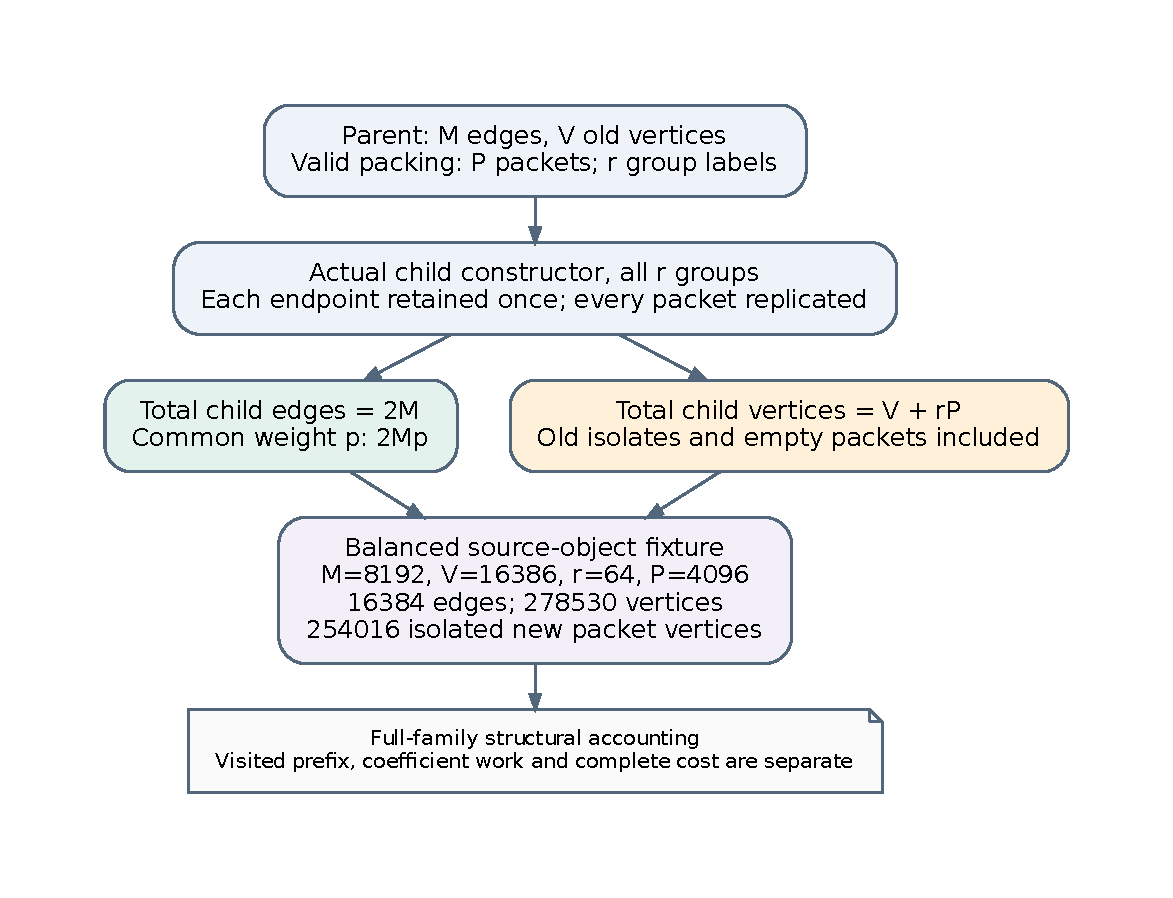
\includegraphics[width=0.95\linewidth,height=3.8in,keepaspectratio]{accounting.pdf}
\end{center}

\textbf{Balanced fixture.} All 64 children have 256 edges, giving 16384 edges.
There are 4096 packets, 262144 new packet vertices, 254016 isolated new packet
vertices, and 16386 old vertices including two old isolates: 278530 vertices
in total. This exposes description/allocation work absent from an edge-only
account. It assigns no timing or asymptotic saving to that work.

\textbf{Consumer boundary.} These counts cover the full constructed group
family. The evaluator may stop on a zero product; its actual visited prefix
is separately bounded. Forced fixtures are not production Setup admission
or a complete contraction evaluation. Coefficient work, mode enumeration,
interpolation and arithmetic widths remain separate cost obligations.

\newpage
{\large\bfseries Controls, qualification and reproducibility}

\begin{tabular}{p{0.49\linewidth}p{0.45\linewidth}}
\toprule
Check & Observed result\\\midrule
One frozen library execution &160 passed; 0 failed/ignored/filtered\\
Base contexts / distinct tuples &2080 / 3388\\
Actual base group constructions &25490, below prospective 46560 cap\\
Balanced groups / negative child probes &64 /6, separate denominators\\
Positive-M wrong-model controls &3128 tuples\\
Final locked offline build / strict Clippy &Pass; all targets, warnings denied\\
Shared / consumer unchanged gates &3 / 3 theorems; 0 trusted native proofs\\
Explicit axiom queries &6, standard foundations only\\
Official fresh kernel replay &\texttt{leanchecker --fresh PortControls},0\\
Raw native rows &3394; 932711 bytes, retained locally\\
\bottomrule
\end{tabular}

The native controls call the real packing, Cauchy, modes, next-tuple and child
routines. Eight geometries, eight edge counts, each coordinate, five graph
families and four label schedules include parallel ports, stars, six-pair
incidence and isolates. They check each group's endpoints, ownership, degree,
old Arc identity and precision 3, new precision 7, vertex counts and prefix
nonnegative edge mass. The separate balanced radix 64 packing enforces native
bounds; z=0 gives no retained modes.

\textbf{Exact errors.} Wrong beta length requires the specific Invalid cause.
Missing/duplicate packet occurrences require their particular Integrity causes.
A valid packing with an exhausted edge budget really returns Limit, which is
excluded from coverage classification. The pre-review v1 was compiled but never
executed; its family/error controls were corrected before the one v2 run.

\textbf{Pins and trust.} Focused qualification uses official Lean 4.35.0 and
Mathlib 56a00585. The unchanged default pin cfc55fc5 is not qualified by this
cache; transitive sources differ even though the counting file matches. All
six axiom queries use only propext, Classical.choice and Quot.sound. No holes,
custom axioms, native\_decide or raised elaboration limits are used. Reviews
are written same-team source checks, not independent execution or signed
standing. Canonical claims are newly appended on the main-based publication
branch; the old divergent producer ledger remains intact locally.

\textbf{Custody.} The 88-file frozen crate includes three pre-existing local
formatting variants in floor\_sum, short\_box and unimodular. Their exact bytes
are retained, but excluded from publication changes. This is not an exact
whole-published-crate qualification. Source/binary pre/post hashes pass; all
raw rows, qualified binary, failed sources and review inputs remain local.

\textbf{Failures and limits.}01/08 had assembly/library-reference failures;
05/07/10 hit the fixed memory stop. Phase 11 passed after compared lossless
archives reclaimed idle storage. One worker, 600s phase ceilings, 120s native
ceiling and 15032385536-byte sampled cgroup stop stayed fixed; phase 11 peaked
at 14816174080 bytes. Administrative parser/path and preparation-sequencing
errors are retained with explicit corrections. No native retry occurred.

\textbf{Reproduction and follow-up.} Restore the exact 88 inputs (including the
three retained variants), Rust1.99.1 and Cargo.lock. Build release/offline/locked,
run strict Clippy, then the copied test binary single-threaded with a fresh
\texttt{PORT\_MASS\_ROWS} path. Signed standing and default-pin integration
remain open. Next bind full source histories/costs and test any proposed unit
packet removal against contraction values and nonunit controls.

\small Sources: primary AppendixD.4.6/D.11 at OpenAI/math42907c9e; actual
constructor at crypto5ec6aed0; existing Mathlib multiset laws. KB unavailable127;
bounded source/GitHub fallback provides no novelty clearance. Canonical runtime
charts remain unchanged for this accounting component. Full proof map,
prospective plans, addenda, receipts and source identities accompany the report.\par
\url{https://github.com/isogeny-labs/crypto/pull/5046}\par
\url{https://github.com/aburan28/crypto-lean/pull/35}
\end{document}
